Consider the following MDP, with three states $B, C$ and $D$ ($\mathcal{S} = \{B,C,D\}$), and 2 actions  ($\mathcal{A} = \{1,2\}$), with $\gamma = 1.0$.
Assume the action values are initialized $Q(s,a) = 0 ~\forall~ s\in\mathcal{S}$ and ~$a\in\mathcal{A}$. The agent takes actions according to an $\epsilon$-greedy policy with $\epsilon = 0.1$. 
\begin{enumerate}
\item What is the optimal policy for this MDP? What are the action-values corresponding to the optimal policy: $q^{*}(s,a)$?
\item Imagine the agent experienced a single episode, and the following experience: $S_0 = B, A_0 = 2, R_1 = 0, S_1 = D, A_1 = 2, R_2 = 4$. What are the Sarsa updates during this episode, assuming $\alpha = 0.1$? Start with state $B$, and compute and apply the Sarsa update. Then compute and apply the Sarsa update for the value of state $D$.
\item Using the sample episode above, compute the updates Q-learning would make, with $\alpha = 0.1$. Again start with state $B$, and then state $D$.
\item \label{ep_2} Let's consider one more episode: $S_0 = B, A_0 = 2, R_1 = 0, S_1 = D, A_1 = 1, R_2 = -100$. What would the Sarsa updates be? And what would the Q-learning updates be?
\item Assume you see one more episode, and it's the same one as in \ref{ep_2}. Once more update the action values, for Sarsa and Q-learning. What do you notice?
\item What policy does Q-learning converge to? What policy does Sarsa converge to?
\end{enumerate}
\begin{figure}[h!]
  \center
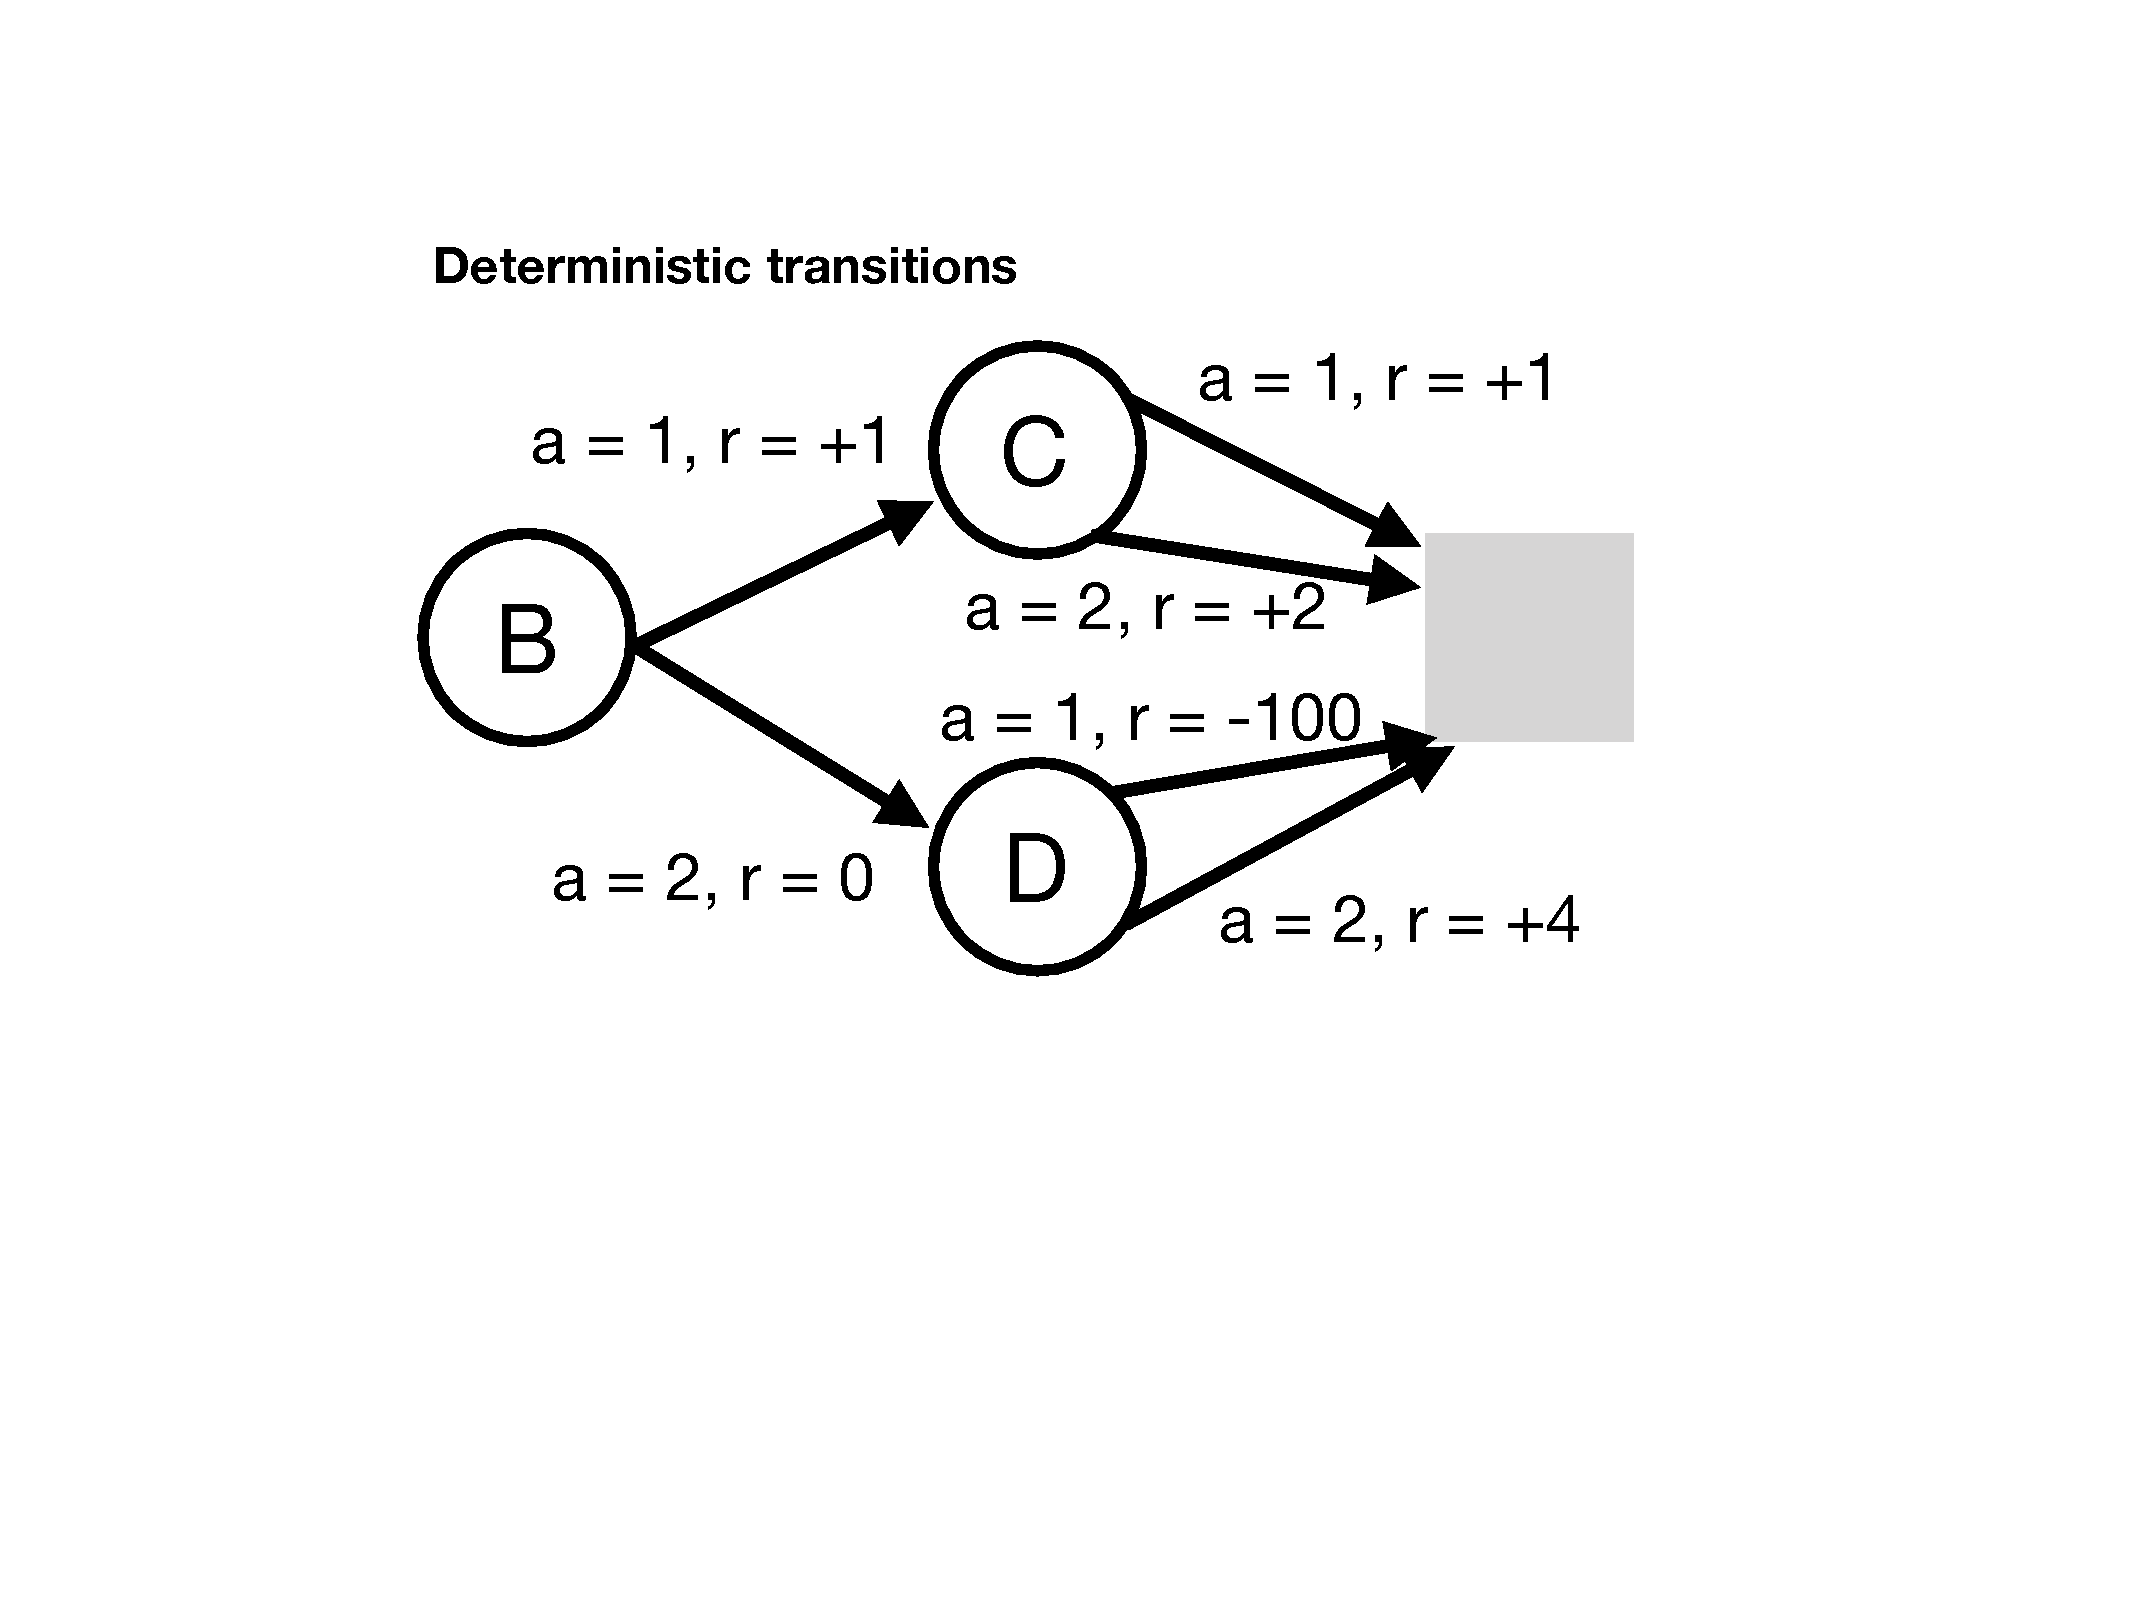
\includegraphics[width=0.5\linewidth]{figures/bcd.pdf}
\end{figure}

%% \textbf{Answer:}
%% \begin{enumerate}
%% \item The Bellman equation for the optimal action value function is $q_*(s, a) = \sum_{s', r} p(s', r|s, a)[r + \gamma \max_{a'} q_*(s', a')]$. Using this, we obtain $q_*(C, 1) = 1, q_*(C, 2) = 2, q_*(D, 1) = -100, q_*(D, 2) = 4, q_*(B, 1) = 1+q_*(C, 2) = 3, q_*(B, 2) = 0+q_*(D, 2) = 4$. The optimal policy is greedy with respect to this value function. So, $\pi_*(2|C) = 1, \pi_*(2|D) = 1, \pi_*(2|B) = 1$ and zero for all other state action pairs.
%% \item  \textbf{SARSA:}

%%   $q(B, 2) = q(B, 2) + 0.1 [0 + \gamma q(D, 2) - q(B, 2)] = 0 + 0.1[0 + 0-0] = 0$, and

%%   $q(D, 2) = q(D, 2) + 0.1 [4 + \gamma q(T, \cdot) - q(D, 2)] = 0 + 0.1[4 + 0-0] = 0.4$.
  
%% \item\textbf{Q--learning:}

%%   $q(B, 2) = q(B, 2) + 0.1 [0 + \gamma \max_{a'} q(D, a') - q(B, 2)] = 0 + 0.1[0 + 0 - 0] = 0$ and

%%   $q(D, 2) = q(D, 2) + 0.1 [4 + \gamma \max_{a'} q(T, a') - q(D, 2)] = 0 + 0.1[4 + 0 - 0] = 0.4$.
  
%% \item
%%   \textbf{SARSA:}
  
%%   $q(B, 2) = q(B, 2) + 0.1 [0 + \gamma q(D, 1) - q(B, 2)] = 0 + 0.1[0 + 0-0] = 0$, and

%%   $q(D, 1) = q(D, 1) + 0.1 [-100 + \gamma q(T, \cdot) - q(D, 1)] = 0 + 0.1[-100  +0-0] = -10$.

%%   \textbf{Q--learning:}

%%   $q(B, 2) = q(B, 2) + 0.1 [0 + \gamma \max_{a'} q(D, a') - q(B, 2)] = 0 + 0.1[0 + 0.4 - 0] = 0.04$ and

%%   $q(D, 1) = q(D, 1) + 0.1 [-100 + \gamma \max_{a'} q(T, a') - q(D, 1)] = 0 + 0.1[-100 + 0 - 0] = -10$.
  
  
%% \item
%%     \textbf{SARSA:}
  
%%   $q(B, 2) = q(B, 2) + 0.1 [0 + \gamma q(D, 1) - q(B, 2)] = 0 + 0.1[0 + -10 -0] = -1$, and

%%   $q(D, 1) = q(D, 1) + 0.1 [-100 + \gamma q(T, \cdot) - q(D, 1)] = -10 + 0.1[-100  +0+10] = -19$.

%%   \textbf{Q--learning:}

%%   $q(B, 2) = q(B, 2) + 0.1 [0 + \gamma \max_{a'} q(D, a') - q(B, 2)] = 0.04 + 0.1[0 + 0.4 - 0.04] = 0.076$ and

%%   $q(D, 1) = q(D, 1) + 0.1 [-100 + \gamma \max_{a'} q(T, a') - q(D, 1)] = -10 + 0.1[-100 + 0 + 10] = -19$.

%%   We observe that the SARSA and Q--learning updates are same for $q(D, 1)$, and they are different for $q(B, 2)$. For $q(B, 2)$, Q--learning makes the update using the next state action pair as $q(D, 2)$ since it has a higher value than the other action value $q(D, 1)$.

%% \item Q--learning converges to the optimal greedy policy. Sarsa converges to the optimal policy in behavior policy class (for example the optimal $\epsilon$--greedy policy). The Cliff Grid World illustrates this.
%% \end{enumerate}
